% Original conceptual figure. Compile standalone or input from the manuscript.
\documentclass[tikz,border=4pt]{standalone}
\usetikzlibrary{arrows.meta,fit,positioning}
\definecolor{airside}{HTML}{2A6F97}
\definecolor{passenger}{HTML}{E07A5F}
\definecolor{energy}{HTML}{8A5A9B}
\definecolor{control}{HTML}{52796F}
\definecolor{ink}{HTML}{374151}
\definecolor{outline}{HTML}{B8C2CC}
\definecolor{metricfill}{HTML}{F4F1DE}
\tikzset{
  box/.style={draw=ink, rounded corners=2pt, align=center, minimum height=8mm, text width=25mm, fill=white},
  flow/.style={-{Stealth[length=2mm]}, thick, ink},
  constraint/.style={-{Stealth[length=2mm]}, dashed, thick, control},
  coupling/.style={-{Stealth[length=2mm]}, thick, passenger},
  group/.style={draw=outline, rounded corners=3pt, inner sep=5mm}
}
\begin{document}
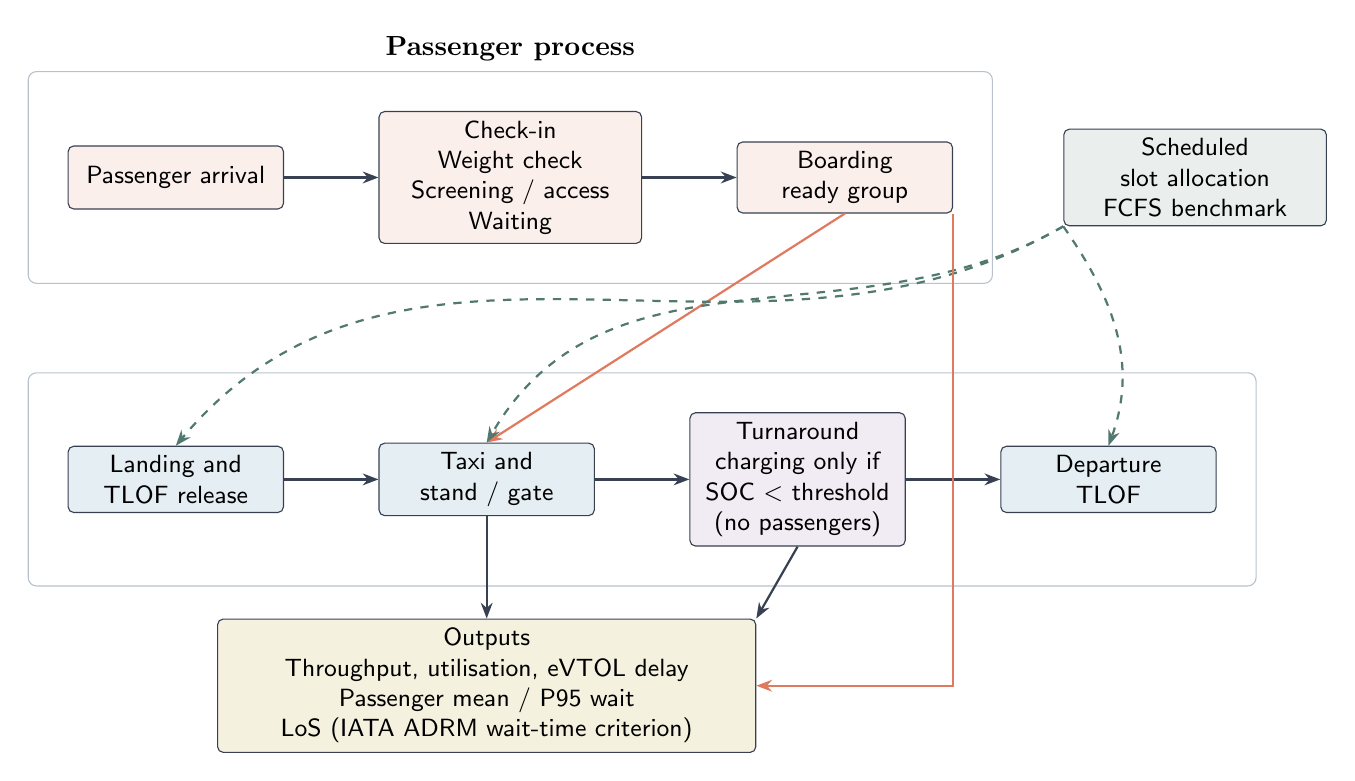
\begin{tikzpicture}[font=\sffamily\small, node distance=9mm and 12mm]
  \node[box, fill=passenger!12] (arrival) {Passenger arrival};
  \node[box, fill=passenger!12, right=of arrival, text width=31mm] (terminal) {Check-in\\Weight check\\Screening / access\\Waiting};
  \node[box, fill=passenger!12, right=of terminal] (boarding) {Boarding\\ready group};
  \node[fit=(arrival)(terminal)(boarding), group, label={[font=\bfseries]above:Passenger process}] (pgroup) {};
  \node[box, fill=airside!12, below=30mm of arrival] (tlofarr) {Landing and\\TLOF release};
  \node[box, fill=airside!12, right=of tlofarr] (stand) {Taxi and\\stand / gate};
  \node[box, fill=energy!12, right=of stand] (turn) {Turnaround\\charging only if\\SOC $<$ threshold\\(no passengers)};
  \node[box, fill=airside!12, right=of turn] (tlofdep) {Departure\\TLOF};
  \node[fit=(tlofarr)(stand)(turn)(tlofdep), group] (agroup) {};
  \node[box, fill=control!12, right=14mm of boarding, text width=31mm] (schedule) {Scheduled slot allocation\\FCFS benchmark};
  \node[box, fill=metricfill, below=13mm of stand, text width=66mm] (metrics) {Outputs\\Throughput, utilisation, eVTOL delay\\Passenger mean / P95 wait\\LoS (IATA ADRM wait-time criterion)};
  \draw[flow] (arrival) -- (terminal);
  \draw[flow] (terminal) -- (boarding);
  \draw[flow] (tlofarr) -- (stand);
  \draw[flow] (stand) -- (turn);
  \draw[flow] (turn) -- (tlofdep);
  \draw[coupling] (boarding.south) -- (stand.north);
  \draw[constraint] (schedule.south west) to[out=-150,in=50] (tlofarr.north);
  \draw[constraint] (schedule.south west) to[out=-150,in=60] (stand.north);
  \draw[constraint] (schedule.south west) to[out=-55,in=70] (tlofdep.north);
  \draw[flow] (stand.south) -- (metrics.north);
  \draw[flow] (turn.south) -- (metrics.north east);
  \draw[coupling] (boarding.south east) |- (metrics.east);
\end{tikzpicture}
\end{document}
